%!TEX program = xelatex
% 完整编译: xelatex -> bibtex -> xelatex -> xelatex
\documentclass[lang=cn,12pt,a4paper,cite=authoryear]{elegantpaper}

% 本文档命令
\usepackage{array}
\usepackage{authblk}
\usepackage{pifont}
\usepackage{threeparttable}
\usepackage{titlesec}
\usepackage{hyperref}
\usepackage{listings}

\newcommand{\sectionbreak}{\clearpage}

\title{大数据场景下语言虚拟机的性能分析与优化调研}

\author{贾兴国, 张正君, 余博识 \\ Shanghai Jiao Tong University \\ \{zhangzhengjunsjtu, 201608ybs, jiaxg1998\}@sjtu.edu.cn}
\institute{\href{http://www.se.sjtu.edu.cn/}{School of Software Engineering}}

\version{1.0}
\date{\zhtoday}



\begin{document}

\maketitle

\begin{abstract}
随着大数据处理系统的快速发展,托管型语言(managed languages)由于其快速的开发周期以及丰富的社区资源得到了广泛的应用。例如,分布式数据处理框架Spark、Hadoop、DryadLINQ、分布式文件系统HDFS、分布式键值存储系统HBase、Cassandra等均使用开发效率较高的Java语言进行开发。托管型语言通过使用语言虚拟机实现对内存的管理,如使用JVM(Java Virtual Machine)进行垃圾回收(garbage collection,GC),免去手动编写代码进行内存释放的需要,也降低了内存管理出现错误的可能。然而,开发的便利性也带来了一定的性能损耗。经过调研,研究者们从不同的角度发现了托管型语言在分布式大数据处理场景下出现的性能问题,如GC时间过长、节点间数据传输太慢、语言虚拟机启动耗时过长等,并且提出了相应的解决方案。本文总结了研究者们发现的问题及其解决方案,并且针对解决方案的局限性与适用性进行了分析,提出了相应的优化方案。
\keywords{语言虚拟机,分布式系统,大数据,垃圾回收}
\end{abstract}

\cleardoublepage
\tableofcontents
\cleardoublepage

\section{研究背景}
随着摩尔定律的终结,单个机器所提供的计算资源已经无法满足海量数据的巨大算力需求。学术界和工业界将关注点从纵向扩展转向了横向扩展,使用多台配置较低的廉价机器代替了配置较高的单台机器,使用分布式系统向数据处理、机器学习、云计算等应用提供可横向扩展的计算资源。运行在分布式系统上的数据处理框架如Spark\cite{spark}、Hadoop\cite{hadoop}、DryadLINQ\cite{DBLP:conf/osdi/YuIFBEGC08}、Naiad\cite{DBLP:conf/sosp/MurrayMIIBA13}等采用了分布式并行的数据处理模式,充分利用分布式集群提供的计算资源。也有分布式文件系统HDFS\cite{hdfs}、分布式键值存储系统HBase\cite{hbase}、Cassandra\cite{cassandra}等利用分布式系统较强的容错性、可扩展性,为数据存储提供了更优的解决方案。

运行在云平台上的分布式软件的快速发展使得托管型编程语言成为了开发人员和研究人员的关注重点。广泛使用的分布式处理框架Hadoop、Spark、Cassandra均使用Java进行开发,DryadLINQ、Naiad等数据处理框架使用由微软开发的C\#语言进行编写。还有更多的托管型语言被广泛使用,如Go、Javascript、Python等。托管型语言如Java、C\#使用语言虚拟机进行自动内存回收,免去了手动编写代码释放内存的需要,还有面向对象的编程风格、丰富的社区资源,使得Java等语言有很高的开发效率。

语言虚拟机带来的开发便捷性建立在一定的性能损耗之上。例如为了运行Java程序,首先对Java源代码进行编译,生成bytecode(字节码),再从classpath中加载、解析、验证字节码文件,以及运行该字节码所需的其他字节码文件,后在JVM中运行字节码。Java语言运行环境(runtime)的加载以及字节码的解释执行相比于Native的编程语言(如C、C++)产生了巨大的开销。同时,Java程序在堆(heap)内存中为对象申请内存,无需手动编写代码释放堆内存,而是使用JVM自带的GC(垃圾回收)功能进行对内存的自动释放。然而,进行GC的过程中,语言虚拟机需要占用应用的CPU资源,或需要应用暂停执行(Stop-the-world),这在延迟敏感的情境下对应用的性能表现有巨大的影响。在分布式数据处理的场景中,由于Java等管理型语言使用在堆上保存的对象(object)来存储、处理数据,GC需要遍历海量的对象,其开销相对于单机、数据量较小的情景也被明显加大。分布式环境下请求的处理依赖于多个节点上的语言运行环境,语言虚拟机的性能优化需要依靠多个语言虚拟机之间的协调,这和单机情境下的语言虚拟机性能优化又大有不同。

本文针对大数据处理场景下的语言虚拟机性能优化进行调研,总结出了分布式大数据处理对语言虚拟机提出的新的挑战,以及研究者所提出的解决方案,并分析了特定解决方案的适用性与优化方案。本文第二章总结了语言虚拟机在大数据情境下表现出的性能问题,以及研究者对相关问题所提出的解决方案。第三章就JVM启动耗时过长问题的研究思路进行了分析,并总结了其局限性与适用范围。第四章提出了针对第三章中适用性问题的解决方案,并搭建原型、验证和测试了解决方案的有效性。在第五章中我们对本文的调研工作进行总结。

\section{大数据场景下语言虚拟机的性能问题与优化}
大数据处理为托管型语言带来了全新的使用场景,同时托管型语言为大数据处理框架带来了较高的开发效率。新的使用情景为托管型语言的语言虚拟机带来了新的挑战。本章对大数据环境下语言虚拟机表现出的性能问题做了总结分析,并对研究者的相应解决方案进行了总结。

\subsection{大数据场景下GC对性能的影响}
\subsubsection{问题概述}
在大数据场景下,应用需要良好的性能与扩展性,然而托管型语言的运行时环境存在臃肿、可扩展性差的问题。语言虚拟机的GC使得应用的主线程必须停止,需要遍历堆中保存的相互引用的复杂的对象,占用大量计算资源,无法进行有用的工作;内存管理模块也有巨大的额外内存开销,虽然所处理的数据量大小比堆内存的容量更小,也会产生OOM(Out Of Memory,内存不足)的报错。但使用非管理型语言会增加应用编写者的负担,更容易出现错误,调试内存管理错误也是一件非常困难的事。当前大量的大数据处理框架已经使用管理型语言进行编写,向非管理型语言的迁移会带来巨大的工作量。故需要有一种方法优化语言虚拟机的GC问题与内存空间占用问题。

\subsubsection{解决方案}
Nguyen等人提出了Facade\cite{DBLP:conf/asplos/NguyenWBFHX15}编译框架。他们认为将大量数据保存在堆内存上,让JVM进行管理是不明智的。通过限制堆内存上保存的对象数量,将数据面与控制面进行分离,仅在堆上保存控制面对象,而数据面中的数据保存在本地内存(native memory)中进行手动管理。这打破了面向对象编程语言的一条规则:对象应当包含数据以及操作数据的接口。对于每一个Java语言中的堆上保存的对象,Facade编译系统生成一个相应的facade,提供对象的操作接口而不保存对象中包含的数据,从而减轻垃圾收集器的负担,而程序员仅需标记出数据类(data class)。对于facade,可以通过对象复用限制堆中对象的数量;而native memory中的数据在每个iteration结束后统一进行释放,无需访问数据的每个字段,相比于垃圾收集器有更优的性能。经测试,Facade使得应用运行时间缩短了48\%,降低了50\%的内存占用。

Gog等人提出了Broom\cite{DBLP:conf/hotos/GogGSVVRCMHI15}内存管理系统,取代了CLR\footnote{CLR\cite{DBLP:conf/indin/CavalieriSG16},Common Language Runtime,是Microsoft .Net框架的语言虚拟机系统、运行时环境,运行.Net程序。使用任何语言编写的.Net程序均运行在CLR上,而JVM仅支持运行Java程序。}的GC系统。他们认为,大数据系统中存在多个Actor,这些Actor独立地运行,它们之间传递消息,形成了高度结构化的数据流,例如MapReduce\cite{DBLP:journals/cacm/DeanG08}中的map工作线程与reduce工作线程。每个Actor内的对象在Actor完成工作后不再会用到,仅有Actor之间传递的数据需要保存,无需GC扫描。为了针对这类高度结构化的应用对垃圾收集器进行优化,Broom内存管理器使用了基于region(分区)的内存管理策略\cite{DBLP:conf/padl/ElsmanH20},对象在各个region中保存而不在堆中由GC管理,由程序员手动释放region中的对象。Broom内存管理器减轻了GC的负担,减少了59\%的运行时间,但使得程序员的负担增加。

\subsection{JVM启动耗时对延迟敏感型应用的影响}
\subsubsection{问题概述}
社区中长期存在对Java性能的激烈讨论,尤其是Java是否适合编写延迟敏感型应用的问题\cite{debate1,debate2,debate3,debate4}。一些程序员坚持使用C++等非管理型语言编写键值存储系统,因为他们认为Java天生就是较慢的。Java之所以适用于编写Hadoop框架是因为Hadoop大部分时间在进行I/O操作\cite{why}。在学术界,对于大数据框架的性能优化主要集中在对GC性能的优化、调度策略的优化、数据交换开销的优化等,故我们缺少对Java各个方面性能的整体了解。经过实验测得,在I/O密集型任务中,JVM的预热开销也是较大的,如在从HDFS中读取1G的文件的过程中,JVM预热使用的时间占总运行时间的33\%b\cite{DBLP:conf/osdi/LionCSZGY16},预热时间不随任务数据量的变化而变化。在大数据框架中,复杂的软件栈使得Java运行环境的加载更加缓慢,因为需要加载更多的class,如Spark为了完成一次请求需要加载19066个class。

\subsubsection{解决方案}
Lion等人经过实验测得,JVM的性能瓶颈在于JVM的启动预热(warm-up),并编写了HotTub\cite{DBLP:conf/osdi/LionCSZGY16}代替了HotSpot\footnote{HotSpot是一个Java虚拟机的实现,由Sun公司开发,包含在OpenJDK中,是主流的JVM。详见https://stackoverflow.com/questions/16568253/difference-between-jvm-and-hotspot}解决了Java虚拟机启动时间过长的问题。他们首先通过修改Java程序的调用过程测量出class加载与字节码解释执行的开销,观察出JVM预热对性能的巨大影响。同时,他们在HotSpot的基础上修改实现了HotTub,在多次请求中复用同一个JVM实例,从而免去JVM的预热开销。

由于大数据应用的相似性,JVM有较大的复用可能,同时频繁使用的字节码在多次复用后被JIT编译成机器码而无需解释执行。HotTub可以让Java程序无修改地运行,免去了JVM的预热开销,使得Spark请求的性能提升到1.8倍。本文将在第三章对Lion等人的HotTub研究进行详细的分析,总结其使用范围与局限性,并在第四章中提出并测试相应的优化方案。

\subsection{分布式环境下多个JVM的协调问题}
\subsubsection{问题概述}
在分布式大数据处理框架中,工作负载运行在多个节点上,即运行在多个相互独立的运行时系统(语言虚拟机)上。这会成为性能降低的原因之一,因为每个运行时系统仅拥有当前运行节点的运行状况,而非全局的分布式应用的运行状,无法做出对全局性能有利的决策。这是之前的工作无法解决的问题,之前的工作仅针对单个节点上的运行时系统进行性能优化。例如,某个节点在不合适的时间进行GC,导致该节点成为整个请求处理流程中最慢的节点。虽然其余节点在较短时间内完成了自己的工作,但仍需等待最慢的节点完成GC,才能将请求结果返回给用户。这将会对延时敏感型与面向吞吐量的应用都造成性能影响。

\subsubsection{解决方案}
Maas等人设计的Taurus\cite{DBLP:conf/asplos/MaasA0K16}系统通过在分布式处理系统中加入一个分布式决策机制,将每个节点上独立的运行时系统组织为一个Holistic Runtime System(全局运行时系统,HRS),从而做出在分布式系统全局下正确的GC、JIT决策。HRS将每个节点上支持分布式应用运行的runtime当做一个整体,看作一个分布式系统,从而做出合理的全局决策,而非每个节点上的runtime独立地做出决策。当在某个节点上运行的一个Holistic Runtime System实例启动时,该实例加入执行同一个policy的runtime的集合,或成为该集合的leader,该集合称为一个coordination group(协调组)。每个实例启动时会附带执行monitor线程,从consensus layer(一致性层)获取本协调组的状态信息。在每个epoch(阶段)结束时,协调组的leader执行该协调组的policy,通过考虑所协调组中所有runtime的状态信息,制定下一个epoch中每个runtime需要执行的事件,同时,协调组中的每个runtime向leader发送自己的最新状态,从而开始下一个epoch。在实验中,作者针对每个分布式应用所遇到的特定问题制定了相应的policy,分别对批处理型工作负载和交互式工作负载进行测试。通过执行STU(Stop The Universe)的policy,批处理型工作负载Spark PageRank的执行时间降低了21\%;对于交互型工作负载Apache Cassandra,read请求的99.99\%的尾延迟从65.7 ms 降低到了 33.8 ms,99.9999\%尾延迟从128.6 ms 降低到了 54.6 ms。

\subsection{大数据场景下节点数据交换的性能问题}
\subsubsection{问题概述}
在大数据系统中,节点间数据的传递是频繁发生的。和之前GC性能问题的根源相同,数据传递也因为需要处理海量的包含着数据的对象(object)而受到了性能影响。数据发送方需要对于Java中的对象(object)进行\textit{serialize}(序列化)才可以在网络中传递,接收方需要将接收到的字节流进行\textit{deserialize}(反序列化)才能生成发送方想要发送的对象。序列化和反序列化严重依赖于Java中的反射机制,这是一个开销较大运行时操作,会严重影响应用的性能;同时程序员需要手写序列化和反序列化函数,较容易出现错误。在堆中使用object管理海量的数据不但会造成巨大的垃圾收集开销,同时因为object中存在的对象头、指向类的指针等产生巨大的额外内存开销。这要求我们进一步考虑Java等面向对象语言中object与数据处理的关系。

\subsubsection{解决方案}
Nguyen等人提出的Skyway\cite{DBLP:conf/asplos/NguyenFNXDL18}将本地与远程的JVM进程中的堆进行连接,使得源节点的堆中的对象无需序列化即可传输到目的节点。作者观察到,在两个JVM之间传输对象只有一个方式,即首先将对象serialize(序列化),将对象转化成一串二进制数据,在网络中传输这段二进制,才能够被另一端的JVM deserialize(反序列化),重新组装成一个object。如果在对象的跨节点传输中直接传输对象,则不存在序列化与反序列化的开销,程序员也无需编写序列化与反序列化对应的函数,减轻了开发负担,减小了出现错误的可能性。Skyway可以在本地与远程JVM进程之间直接传送object,源节点将对象直接写入output buffer(放置于native memory中),通过网络将对象写入目的节点位于JVM堆中的input buffer,对象无需反序列化即可使用。在对Spark PageRank和TriangleCounting程序的测试中,由于出现了大量的节点间数据交换,Skyway节省了大量序列化和反序列化的时间,比默认Java Serializer快36\%,比Kryo\cite{kyro}快16\%。

Navasca等人认为,数据分析的任务经常使用的数据类型是不可变且被限制的,他们开发的Gerenuk\cite{DBLP:conf/sosp/NavascaCNDLKX19}编译器将一个SER(speculative execution region,预测执行区)编译为直接对来自于磁盘或网络的native bytes进行操作的代码,从而降低了object表示数据所产生的额外内存开销,同时减小了运行时开销、垃圾回收开销与序列化、反序列化开销。与Skyway不同,Gerenuk更希望数据以native bytes存在,这样有多方面的优势,如GC负担减小、object额外开销减小、序列化、反序列化开销减小。由于SER开始于一个反序列化点,终止于一个序列化点,Gerenuk需要大数据框架开发者标记出这些起始点与终结点。通过将object编译为处于native memory中的数据结构、细粒度地将Java bytecode编译为访问native memory的指令,Gerenuk获得了更低的GC开销与序列化、反序列化开销。Gerenuk编译的Spark、Hadoop程序均获得了更低的内存占用、更低的GC开销、序列化、反序列化开销等。

\subsection{资源解聚架构下的GC算法优化}
\subsubsection{问题概述}
在大数据处理集群中,资源碎片化问题影响着集群资源使用率,如内存资源,单个节点不一定在全部的时间段都对内存有较高的利用率。当内存利用率较低时,单机上的空余内存无法被集群中其他节点所利用,即出现了资源碎片化的问题。资源解聚架构的出现解决了这一问题,与普通的单体服务器(monolithic servers)不同,资源解聚架构的数据中心中每个server仅负责对集群提供单一的一种资源,如内存服务器提供内存资源。这类架构使得某种资源可以被多个节点的进程使用,避免了资源碎片化问题;单个节点的崩溃不会影响整个系统,仅会使得某种资源的可用余量减小,提高了系统的容错能力,同时也提高了系统的可扩展性,可以方便地引入新的资源服务器扩充资源量。

对于内存资源,虽然RDMA大大降低了访问远程内存的吞吐量与延迟,但是访问远程节点的内存仍然是一个耗时操作,具有良好的内存访问局部性的(locality)应用程序才能够高性能地运行在资源解聚架构中。然而大数据场景下经常使用的管理型语言则不能表现出良好的内存访问局部性。GC需要遍历堆中的所有object来查找不可达的对象,是一个典型的图计算型工作负载,不具有局部性。同时,类似Java的管理型编程语言使用指针连接各种对象,这也不具有局部性。例如Spark中的RDD\footnote{RDD,Resilient Distributed Datasets\cite{DBLP:conf/nsdi/ZahariaCDDMMFSS12},是Spark的核心数据结构,是一组可以被并行操作的可容错的分布式数据集,保存在内存中。},在资源解聚架构下,遍历一个RDD需要访问多个内存服务器。管理型语言的运行时需要对资源解聚架构进行适配优化。

\subsubsection{解决方案}
Chenxi Wang等人开发的Semeru\cite{semeru}是一个分布式的JVM,可以支持Java程序无修改地运行在资源解聚架构的集群中,通过将GC的object tracing、内存释放等工作卸载到内存服务器上,从而在GC时获得更好的并行性和局部性。为了实现一个资源解聚架构友好的JVM,需要解决三个问题:

一是应当提供怎样的内存抽象。由于需要将GC卸载到内存服务器上,则需要在内存服务器上运行一个对象管理进程(如JVM),那么同一个object在CPU服务器上的内存虚拟地址则与内存服务器上的不同。Semeru提供了一个统一Java堆(Universal Java heap,UJH)对于CPU 服务器上的main进程可以看到一个连续的统一的虚拟地址空间,存放着它操作的对象,而该main进程的辅助进程运行在各自的内存服务器上,可以看到并管理统一虚拟地址空间的一部分。

二是应当将什么工作移交到内存服务器上进行。GC中仅有跟踪对象(tracing objects)这一工作可以与应用程序无错误地并行运行,而移动、释放对象则需要应用程序停止才可以保证正确性。Semeru不断地跟踪其负责的对象,不论CPU 服务器是否需要进行GC,也能够利用到各类硬件加速器。当需要对象的清理与释放时,内存服务器向CPU服务器发送请求,停止CPU服务器上的应用程序(stop-the-world),但这也为内存服务器将对象重新布局从而增强内存访问局部性提供了机会。

三是如何高效地进行swap。目前的swap系统尚未对语言运行时进行适配,如在Infiniswap\cite{DBLP:conf/nsdi/GuLZCS17}上运行Spark会报错。Semeru修改了NVMe-oF的实现从而实现了高效的远程内存访问,同时添加了system call使得语言运行时能够高效地与swap系统进行交互。

Semeru使得Spark和Flink在资源解聚系统上获得了较大的性能提升,端到端性能在CPU服务器cache大小是50\%、25\%的heap大小的情况下分别提升了2.1倍、3.7倍,应用性能提升1.9倍、3.3倍,GC性能提升4.2倍、5.6倍。

\subsection{相关工作小结}
本章对语言虚拟机在大数据情景下遇到的问题做了总结,并针对每个问题分类、总结了相关研究工作的基本思想与原理。

语言虚拟机在大数据环境下需要大量的对象对数据进行管理,这会造成内存开销过大、GC耗时过长的问题。Facade将Java程序中的数据面和控制面分开,从而将对象从heap(堆)中移动到native memory中,达到了优化目的,但有极大的开发难度,无法使用在真实生产环境下。

Broom则关注了object的明确的生命周期,使用region-based的内存管理策略,为用户提供手动分配、释放数据对象的接口,但仅仅适用于Naiad开发者,且没有提供自动化支持,开发负担较大。Yak\cite{DBLP:conf/osdi/NguyenFXDLAM16}也关注到了大数据环境下数据对象的生命周期,通过使得GC算法适应于数据对象的生命周期,减小了GC的开销,但没有解决object造成的内存膨胀问题与序列化、反序列化问题。

Skyway和Gerenuk则关注了大数据环境下节点间数据交换的问题,Skyway直接在节点之间传输object,省略了数据的native bytes格式,但没有解决object额外内存开销过大的问题;Gerenuk则将Java字节码编译为直接操作native bytes的语句,使得数据不以object形式存在,从根本上解决了之前研究成果遇到的问题。

针对语言虚拟机的大量优化仅关注了单机上的语言虚拟机的优化,没有关注全局的运行情况对语言虚拟机的影响。Taurus使用Holistic Runtime System对分布式系统中每个节点上的heap进行管理,通过监控每个节点的运行情况,在合适的时间进行GC,使得垃圾回收不影响分布式应用的性能。

Semeru则关注内存解聚架构下的语言虚拟机GC性能问题。内存解聚架构由于其较好的可扩展性、容错性而越来越受到关注,然而这类架构需要应用有较好的内存访问局部性,管理型语言的GC却是一个图计算类型的工作负载,不具有局部性。Semeru将GC卸载到内存服务器上,提高了GC的内存访问局部性,使得管理型语言更适用于资源解聚架构。

\begin{table}
  \centering
	\caption{相关研究工作对比}		
	\label{compare}
	\resizebox{\columnwidth}{!}{
  \begin{tabular}{c|cccccccc}
    \toprule[1.5pt] % 设置顶线的粗细
    对比项 & Facade &Broom& Taurus& HotTub &Skyway&Gerenuk& Yak & Semeru\\
    \midrule[1.5pt]
    发表会议	& ASPLOS  & HotOS & ASPLOS & OSDI & ASPLOS & SOSP & OSDI & OSDI\\
		\hline                                       
		发表年份	& 2015  & 2015 & 2016 & 2016 & 2018 & 2019 & 2016 & 2020\\
		\hline                                       
		% \rule{0pt}{10pt} % 15pt代表行宽
		减轻GC负担& \ding{51} & \ding{51} & \ding{55} & \ding{55} & \ding{55} & \ding{51} & \ding{51} & \ding{55}\\
		\hline                                        
		% \rule{0pt}{10pt}
	  减少S/D\footnotemark[1]操作	& \ding{55} & \ding{55} & \ding{55} & \ding{55} & \ding{51} & \ding{51} & \ding{55} & \ding{55}\\
		\hline
		% \rule{0pt}{10pt}
    控制/数据面分离 & \ding{51} & \ding{51} & \ding{55} & \ding{55} & \ding{51} & \ding{51} & \ding{51} &\ding{55} \\
    \hline
		% \rule{0pt}{10pt}
    关注对象lifetime & \ding{55} & \ding{51} & \ding{55} & \ding{55} & \ding{55} & \ding{55} & \ding{51} &\ding{55} \\
    \hline
		% \rule{0pt}{10pt}
    无需手动修改应用& \ding{55} & \ding{55} & \ding{51} & \ding{51} & \ding{55} & \ding{51} & \ding{55} &\ding{51} \\
    \hline
		% \rule{0pt}{10pt}
    缩短JVM预热时间 & \ding{55} & \ding{55} & \ding{55} & \ding{51} & \ding{55} & \ding{55} & \ding{55} &\ding{55} \\
    \hline
		% \rule{0pt}{10pt}
    运行时系统间协调 & \ding{55} & \ding{55} & \ding{51} & \ding{55} & \ding{55} & \ding{55} & \ding{55} &\ding{55} \\
    \hline
		% \rule{0pt}{10pt}
    资源解聚架构GC & \ding{55} & \ding{55} & \ding{55} & \ding{55} & \ding{55} & \ding{55} & \ding{55} &\ding{51} \\
    \hline
		% \rule{0pt}{10pt}
		基于JVM & \ding{51} & \ding{55} & \ding{51} & \ding{51} & \ding{51} & \ding{51} & \ding{51} &\ding{51} \\
		\bottomrule[1.5pt]
	\end{tabular}}
\end{table}

\footnotetext[1]{指Serialization序列化/Deserialization反序列化}

HotTub则关注JVM启动预热的开销问题。大数据框架中的延迟敏感型任务会因为管理型语言固有的性能问题而受到影响。研究者认为,语言虚拟机的预热加载过程是管理型语言性能问题的根源所在,HotTub通过在内存中保留前次请求的JVM进程数据,从而免去了类加载、字节码解释执行的开销,但也加大了内存开销。

本章总结的工作较大部分集中在如何降低Java使用对象保存、管理数据的开销上,也有关注分布式系统下各个节点上语言运行时的协调问题,以及语言运行时的预热问题,较大程度上解决了语言运行时在大数据场景下表现出的性能问题。各类研究的对比见表 \ref{compare}。

\section{HotTub研究思路分析}
管理型语言相比于非管理型语言存在着语言运行时带来的额外开销。如Java语言,虽然无需程序员手动释放内存,JVM进行自动GC,降低了应用程序的开发复杂度以及出错的可能,但需要垃圾回收。语言虚拟机的性能优化研究有较高的热度,尤其是大数据时代的到来,使得管理型语言的应用范围更加广阔。然而,已有的研究成果大部分集中于优化垃圾回收、shuffling的优化、以及调度优化等,但尚未对Java程序运行的整个过程中可能造成性能下降的部分有过研究。Lion等人通过对Java工作负载的运行时间分解得出,Java虚拟机(Java Virtual Machine,JVM)的预热占用了Java应用程序的大量运行时间,且JVM预热时间对延迟敏感型应用的响应时间有很大的影响。Lion等人实现了HotTub\cite{DBLP:conf/osdi/LionCSZGY16},在多次请求中复用同一个长时间运行的JVM,从而消除了JVM的预热开销,提高了交互式应用的性能。本章对HotTub的研究思路进行分析,并对其设计与实现进行介绍、测试了其带来的性能提升。

\subsection{延迟敏感型应用中Java的性能问题}
近年来,latency-sensitive(延迟敏感型)的交互型大数据应用受到广泛关注,例如Hive\cite{hive},是建立在Hadoop上的数据仓储系统,向用户提供类似于SQL的数据访问接口,掩盖了底层的分布式架构的复杂性,学习成本较低,且使得传统的SQL编写的应用更容易移植到分布式系统上,获得分布式系统所带来的好处。HiveQL是Hive提供的数据库请求语言,当用户使用HiveQL向Hive发出query(请求),Hive将用户请求转化为MapReduce、Apache Tez\cite{tez}或Spark的jobs。类似的SQL query引擎还有Impala\cite{impala}、Spark SQL\cite{DBLP:conf/sigmod/ArmbrustXLHLBMK15}等。相比于批处理型任务,SQL query需要更低的请求时延,故需要较高的性能。

然而,开发者们认为Java语言天生运行速度慢。例如,Hypertable\cite{DBLP:conf/aaai/RiosJ11}的开发者使用C++是因为Java在延迟敏感的环境下表现不佳,而Hadoop框架使用Java语言编写是因为其大部分工作是I/O处理。Hypertable是一个内存密集型的程序,频繁调用malloc,且需要大量的内存,内存不足会导致内存中的数据溢出到磁盘上,造成较大的性能影响。而Java的内存管理性能比C++差2到3倍,这使得malloc的性能无法保证,且Java对象管理需要额外的内存开销,与Hypertable中的数据争夺内存空间。

也有开发者认为,只要运行环境的CPU、内存资源充足,并且将运行时间较长的任务改写为并行度较高的、较短的任务,那么JVM造成的开销就可忽略不计。如果系统中有充足的内存,则GC的负担将会很小,即使需要GC,也可以使用空闲的CPU资源而不抢占应用程序的CPU资源。JVM的性能也与应用程序的特性有关,如果应用程序有一小部分频繁执行的代码,则会被JIT(Just In Time)编译器编译为机器码而无需JVM解释执行。前面所述的各类性能问题需要通过对Java程序的运行进行全局的统计测试,才可以找出真正的性能瓶颈,得知为什么Java会对延迟敏感型的大数据应用造成性能影响。

\subsection{JVM预热开销测试与分析}
\subsubsection{主要发现}
是什么导致开发者们普遍认为Java比C/C++更慢?经过在JVM中加入计时代码,记录应用各个部分的执行时间,研究者发现JVM的预热占据了整个执行时间的较大部分。JVM的预热指class loading\cite{loading}(类的加载)\footnote{JVM从classpath中按需加载应用程序所需的class,从磁盘上读取.class文件进入内存,并进行初始化。},以及bytecode interpretation\cite{interpreted}(字节码的解释执行)。

\paragraph{I/O密集型应用也有较大的JVM预热开销} JVM的预热开销在I/O密集型的工作负载中依然十分显著,从HDFS中读取1G的数据需要花费33\%的时间进行JVM预热,同时Java字节码的解释执行也有巨大的开销,例如作为HDFS读取的性能瓶颈的CRC checksum计算,当JIT将其代码编译成机器码后有了230倍的性能提升,而只有频繁被执行的代码段才会被JIT系统编译为机器码。

\paragraph{JVM的预热开销不会随着任务的运行时长变化} Spark请求处理需要的JVM预热需要21秒,无论工作量的大小如何变化。这意味着,通过提高程序并行度从而优化程序性能(即将运行时间长的工作负载切分成可以并行运行的运行时间较短的工作负载)的方法因为JVM预热的开销较大而不再可行,甚至需要向另一个方向发展,即延长程序的运行时间,从而减小JVM预热时间占程序运行时间的比例。

\paragraph{复杂的软件栈进一步加大了JVM预热开销} 虽然大数据框架提高了开发效率,简化了开发过程,但这建立在复杂的软件栈之上。例如,Spark处理请求需要加载19066个class,而Hive软件栈较为简单,仅需加载相比于Spark三分之一的class。同时,由于Spark处理请求依赖的class较多,Spark更容易调用一些很少调用的函数,这些函数只能够解释执行,这进一步增加了JVM的预热开销。但由于大数据处理框架的homogeneity(同质性),这些类和函数会在不同的请求之间复用,这为我们提供了优化的可能。

\subsubsection{JVM预热开销的测量}
为了更加准确地测量JVM在主流的工作负载下的预热开销,研究者在JVM代码中添加计时代码,从而测量单个线程中class loading以及bytecode interpretation的耗时。其中class loading已有工具可以统计一段时间内某个JVM进程的class loading情况,包括加载、卸载的class数目以及内存大小、加载卸载class所用的时间,只需将class loading的状况改写为thread local进行统计即可。

而测量bytecode interpretation的耗时较为困难。JVM代码有三种执行的模式:JVM解释执行,JIT编译执行,以及执行C/C++语言的native代码。为了测量JVM解释执行bytecode的耗时,需要对执行模式转换进行标记,我们需要关注的模式转换有从JVM解释执行转换到JIT编译执行,以及从JIT编译执行转换到JVM解释执行。而这两种执行模式的转换发生在\textbf{\texttt{call}}指令和\texttt{ret}指令执行之时。对于\texttt{call}指令,如bytecode调用JIT编译好的代码,或JIT编译好的代码调用bytecode代码,问题比较简单,由于这样的调用必须首先经过一个adapter。对于一个Java中的函数,都有一个\texttt{Method}结构体与之对应,其中包含了解释执行的字节码的入口点,以及JIT编译的机器码的入口点,还有\texttt{i2c}、\texttt{c2i}两个adapter分别供bytecode调用JIT编译好的代码、JIT编译好的代码调用bytecode代码。adapter的存在是由于两种执行模式的calling convention不同,即函数间传递参数的约定不同,它提供了标记执行模式转换的机会。而对于\texttt{ret}指令,则没有这样的标记机会。\texttt{ret}指令仅仅将栈顶的返回地址弹出,并执行返回地址处的代码,没有标记的机会。

\begin{figure}[!htp]
  \centering
  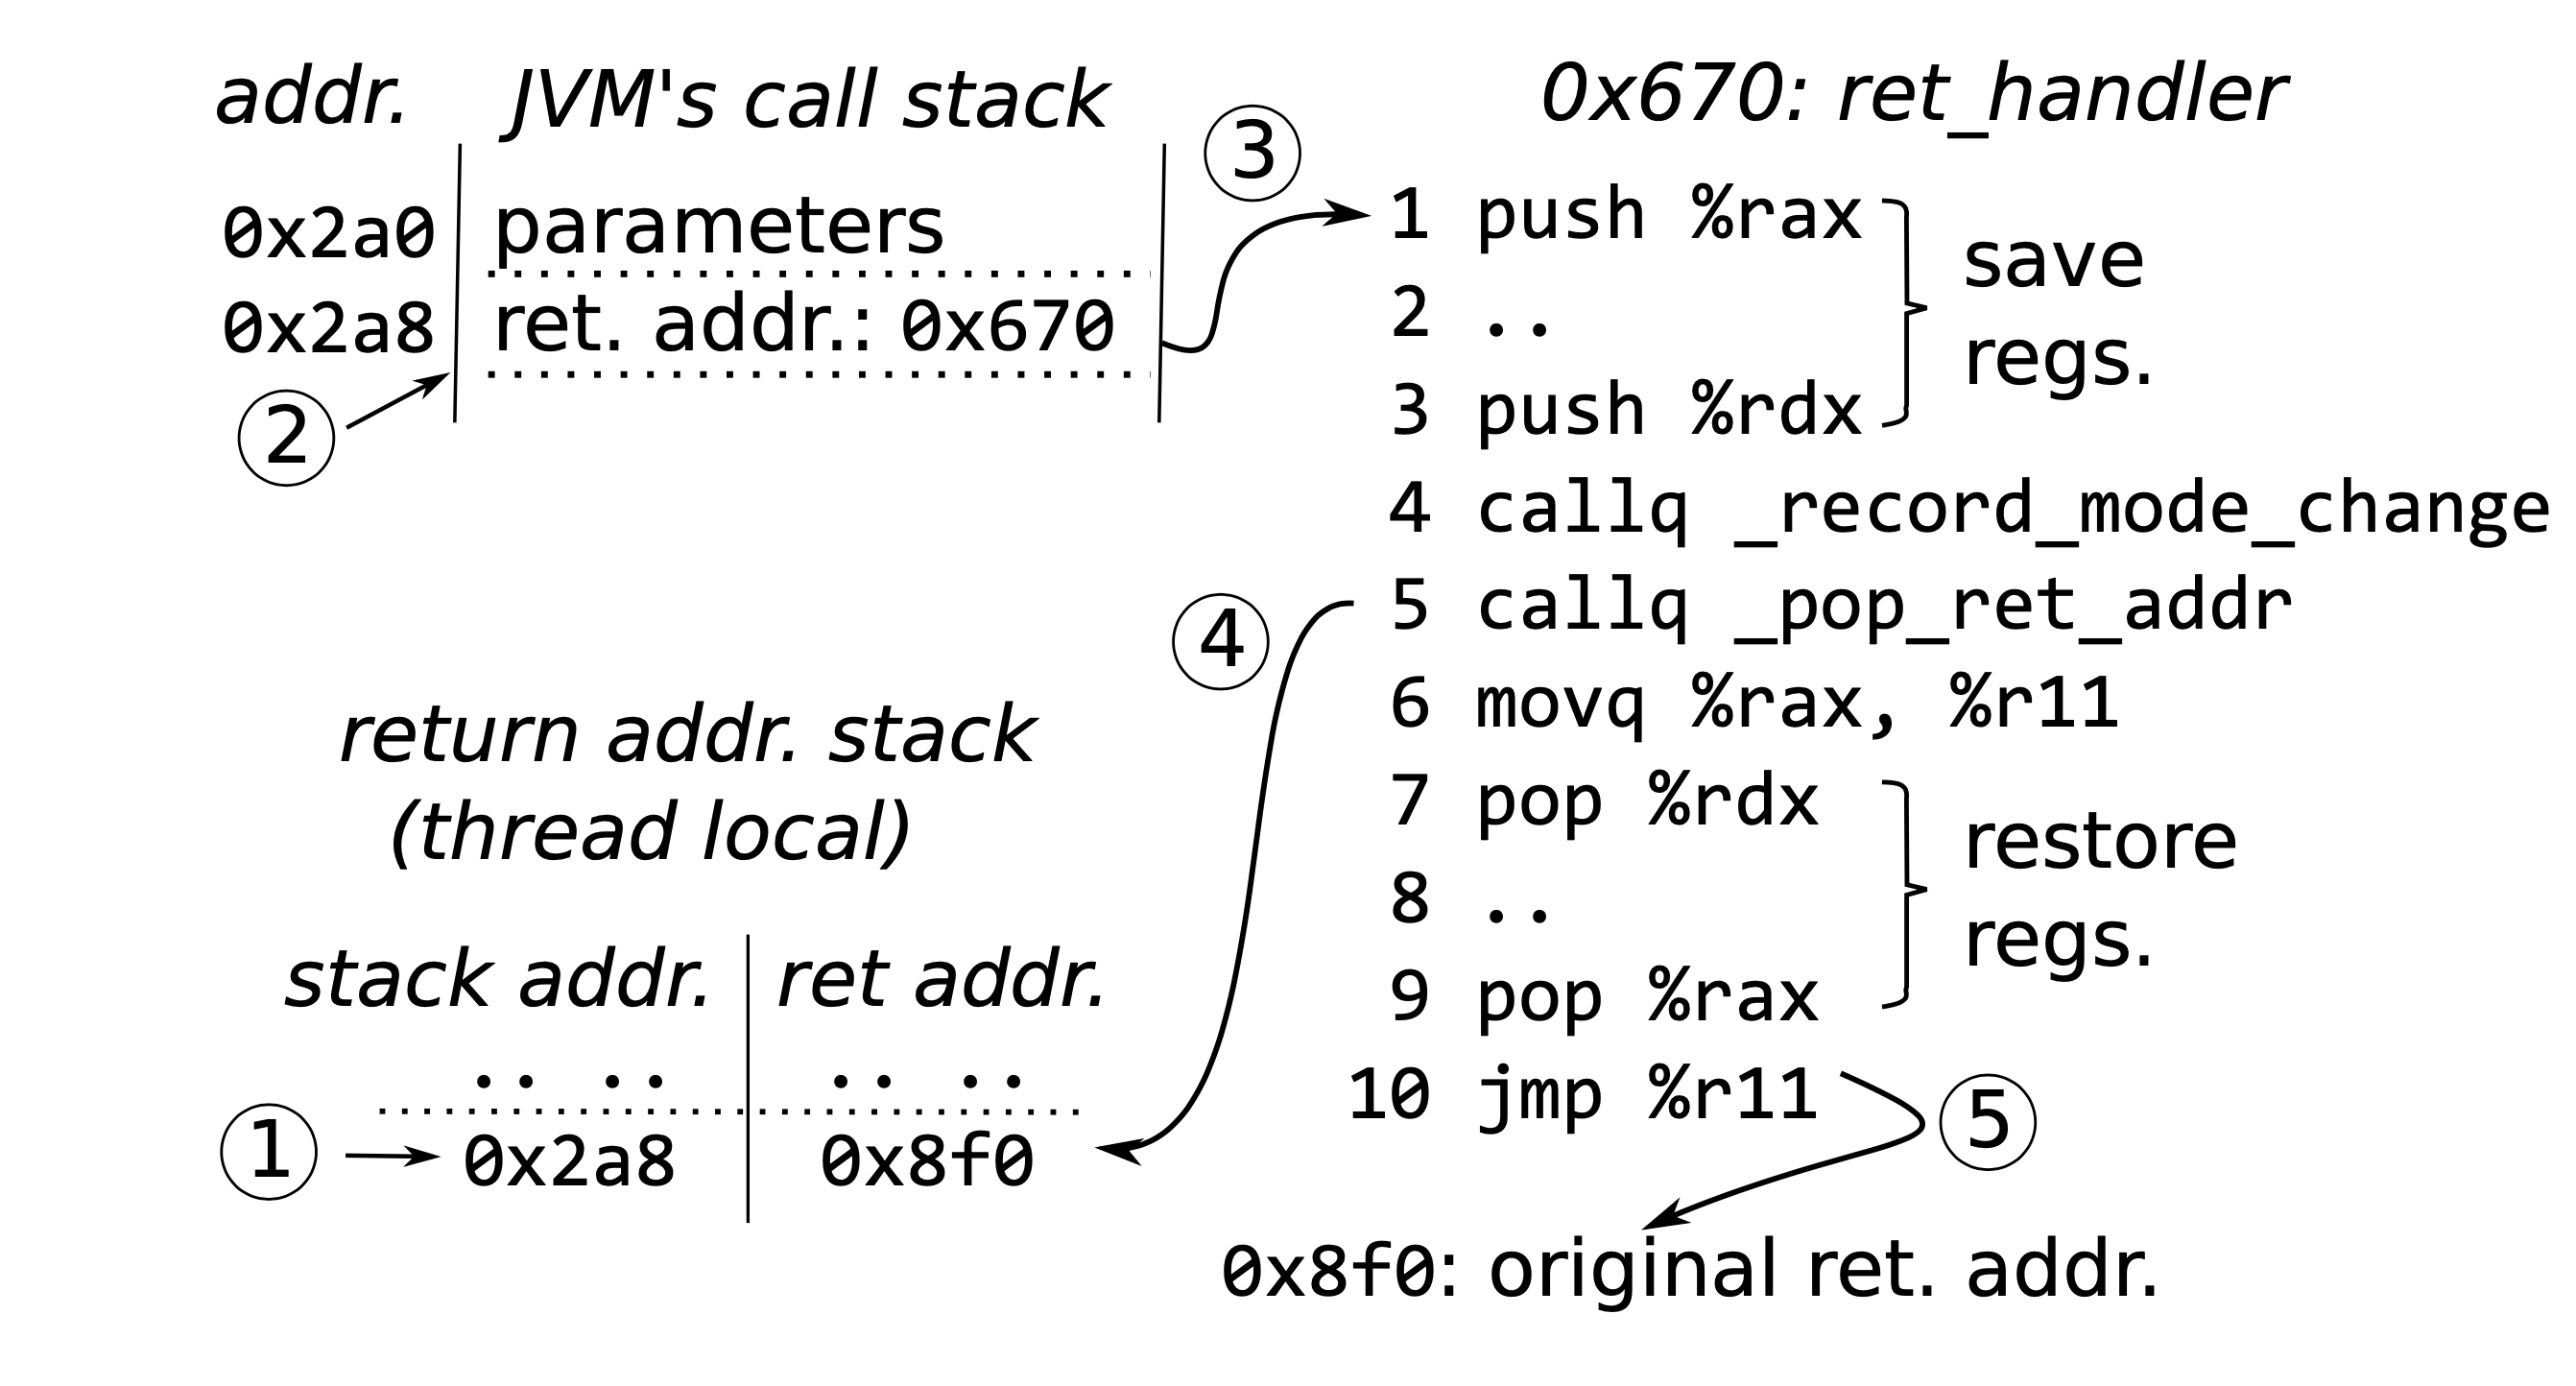
\includegraphics[width=10cm]{1-intercept.png}
  \caption{截获\texttt{ret}指令的执行模式切换}
  \label{fig:intercept}
\end{figure}

故需要对\texttt{ret}指令进行特殊处理。如图\ref{fig:intercept},其主要思想是将\texttt{ret}指令保存在栈上的返回地址修改为自定义的函数,通过5个步骤实现。(1) 每当引发执行模式切换的\texttt{call}指令执行时,进行标记,同时将原有的返回地址保存在一个thread-local的栈上;(2) 将原有的返回地址(\texttt{0x8f0})替换为\texttt{ret\_handler}的地址(\texttt{0x670:ret\_handler}),使得\texttt{ret}指令执行后返回到\texttt{ret\_handler}函数;(3) \texttt{ret\_handler}函数保存所有的寄存器,并调用\texttt{\_record\_mode\_change}记录一次执行模式转换;(4) 调用\texttt{\_pop\_ret\_addr}得到原有的返回地址(\texttt{0x8f0}),保存在\texttt{\%r11}寄存器中;(5) 恢复所有的寄存器,并且跳转到原有的返回地址,完成原有\texttt{ret}指令的功能。\texttt{ret\_handler}的实现使用了15行汇编代码。

但是,修改返回地址在一些corner cases下会产生错误,例如GC使用返回地址寻找caller。在GC开始时,复原全部的返回地址,从而使得GC正常工作。Java语言的异常追踪也依赖于返回地址,故在抛出一个异常之前也需要复原全部的返回地址。JVM的标记仅造成了微小的性能开销,当class loading和bytecode interpretation的注释全部开启时,HDFS的工作负载仅受到了3.3\%的性能影响。

\begin{figure}
  \centering
  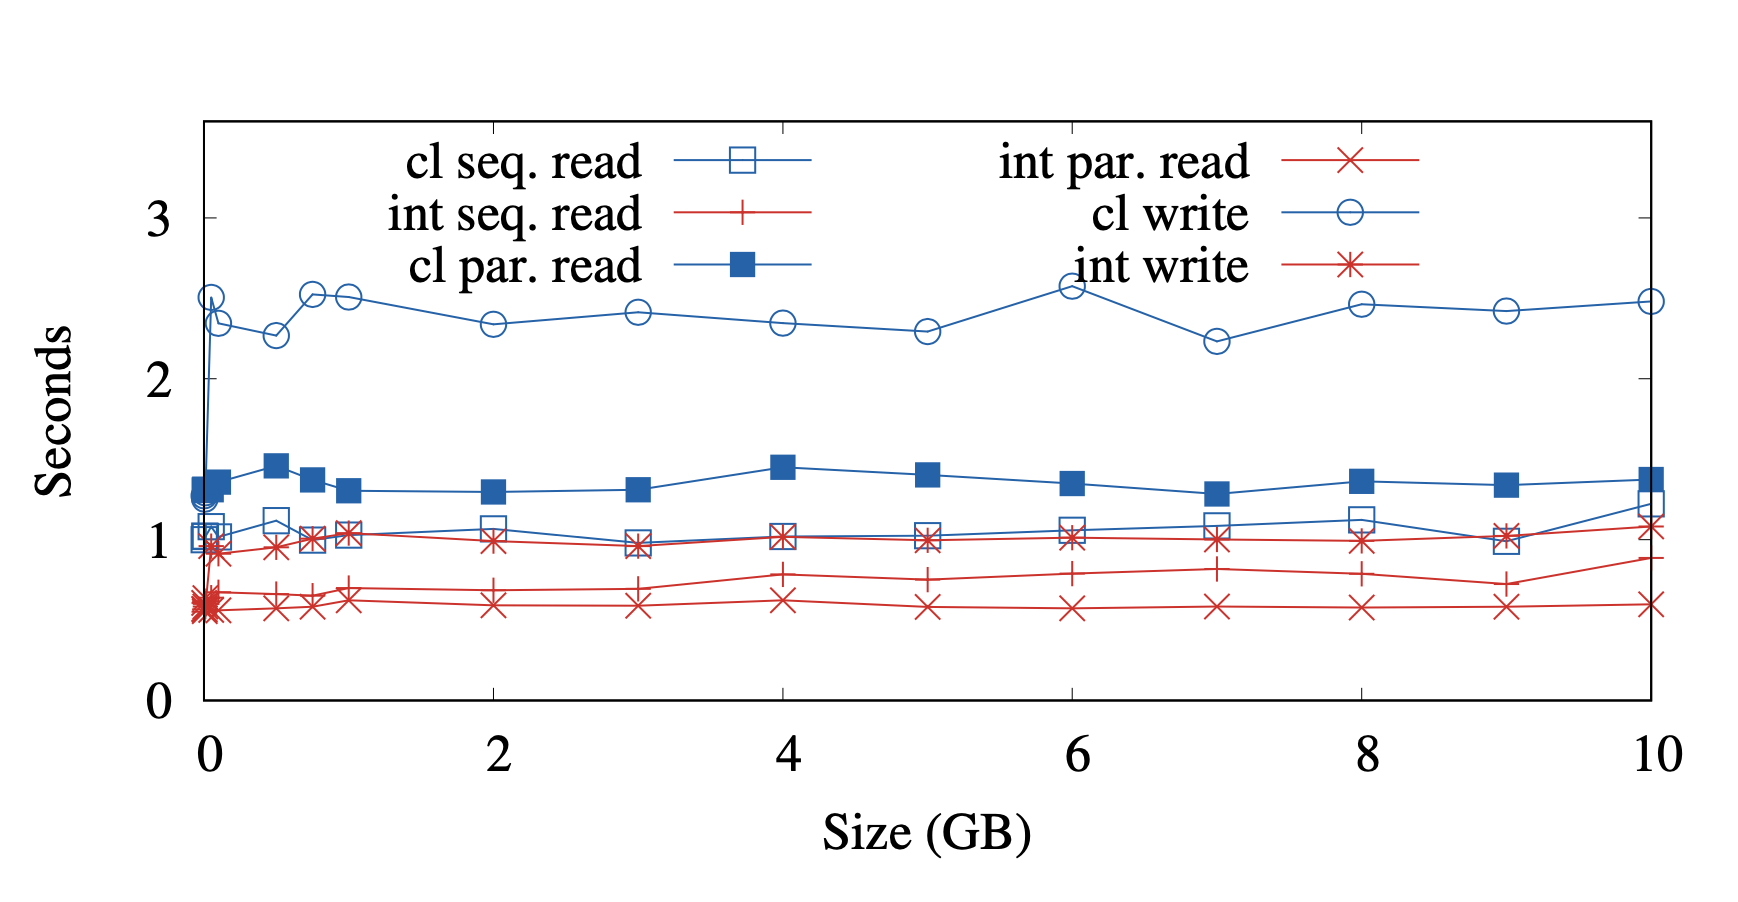
\includegraphics[width=10cm]{2-time.png}
  \caption{HDFS请求预热耗时时长}
  \label{fig:time}
\end{figure}

\subsubsection{JVM预热开销分析}
\label{sec:exe}
借助上一章中的JVM标记,本节对广泛使用的延迟敏感型大数据框架Hive\cite{hive}、Spark SQL\cite{DBLP:conf/sigmod/ArmbrustXLHLBMK15}以及分布式文件系统HDFS\cite{hdfs}进行JVM预热开销分析。Hive和Spark SQL是广泛使用的并行数据处理框架,运行在分布式文件系统HDFS上,它们将用户请求分解成为多个并行运行的较短的jobs进行处理。在Spark中,所有的短jobs运行在同一个JVM进程(\textit{executor})中,每个JVM线程运行一个job;而在Hive中,每个job运行在一个独立的JVM进程中。本文使用BigBench\cite{DBLP:conf/sigmod/GhazalRHRPCJ13}对Spark SQL和Hive进行测试,它包含了30个结构化的、半结构化的、非结构化的数据请求,均来自于真实环境,被Cloudera、Horton-works等公司用于其优化方案。本节测试运行在由10个服务器组成的室内集群中,它们通过10Gbps的网络相互连接。服务组件在测试前经过数周的预热和上千次的试运行。

对于Spark,实验测试了100, 300, 500, 700, 1K, 2K, 3K共7个数据量的请求,Hive则测试了100, 300, 500, 700, 1K共5个数据量的请求,其单位是1G(如100的测试量代表请求100G的数据)。每个请求运行10次,且只取请求时间最短的一次的测试结果,这是为了避免同一个服务器上运行的其他线程(如GC、JIT线程,还有其他操作系统中的线程)对请求性能的影响,最真实地反应请求的时延。同时,由于BigBench测试的方面比较全面,包含了各种真实环境下可能出现的业务请求,其中包含了一些运行时间较长的请求,不属于延迟敏感型请求,作者只测试了BigBench中完成时间最短的10个请求(编号为1, 9, 11, 12, 13, 14, 15, 17, 22, 24),作者关注的重点是latency sensitive的请求。JVM标记仅测量了每个线程中的JVM预热耗时,却没有测量整个进程中JVM预热所占用的时间,作者使用Ousterhout等人提出的估算方法估算出了JVM预热在整个并行程序中所占的运行时间。

\begin{figure}
  \centering
  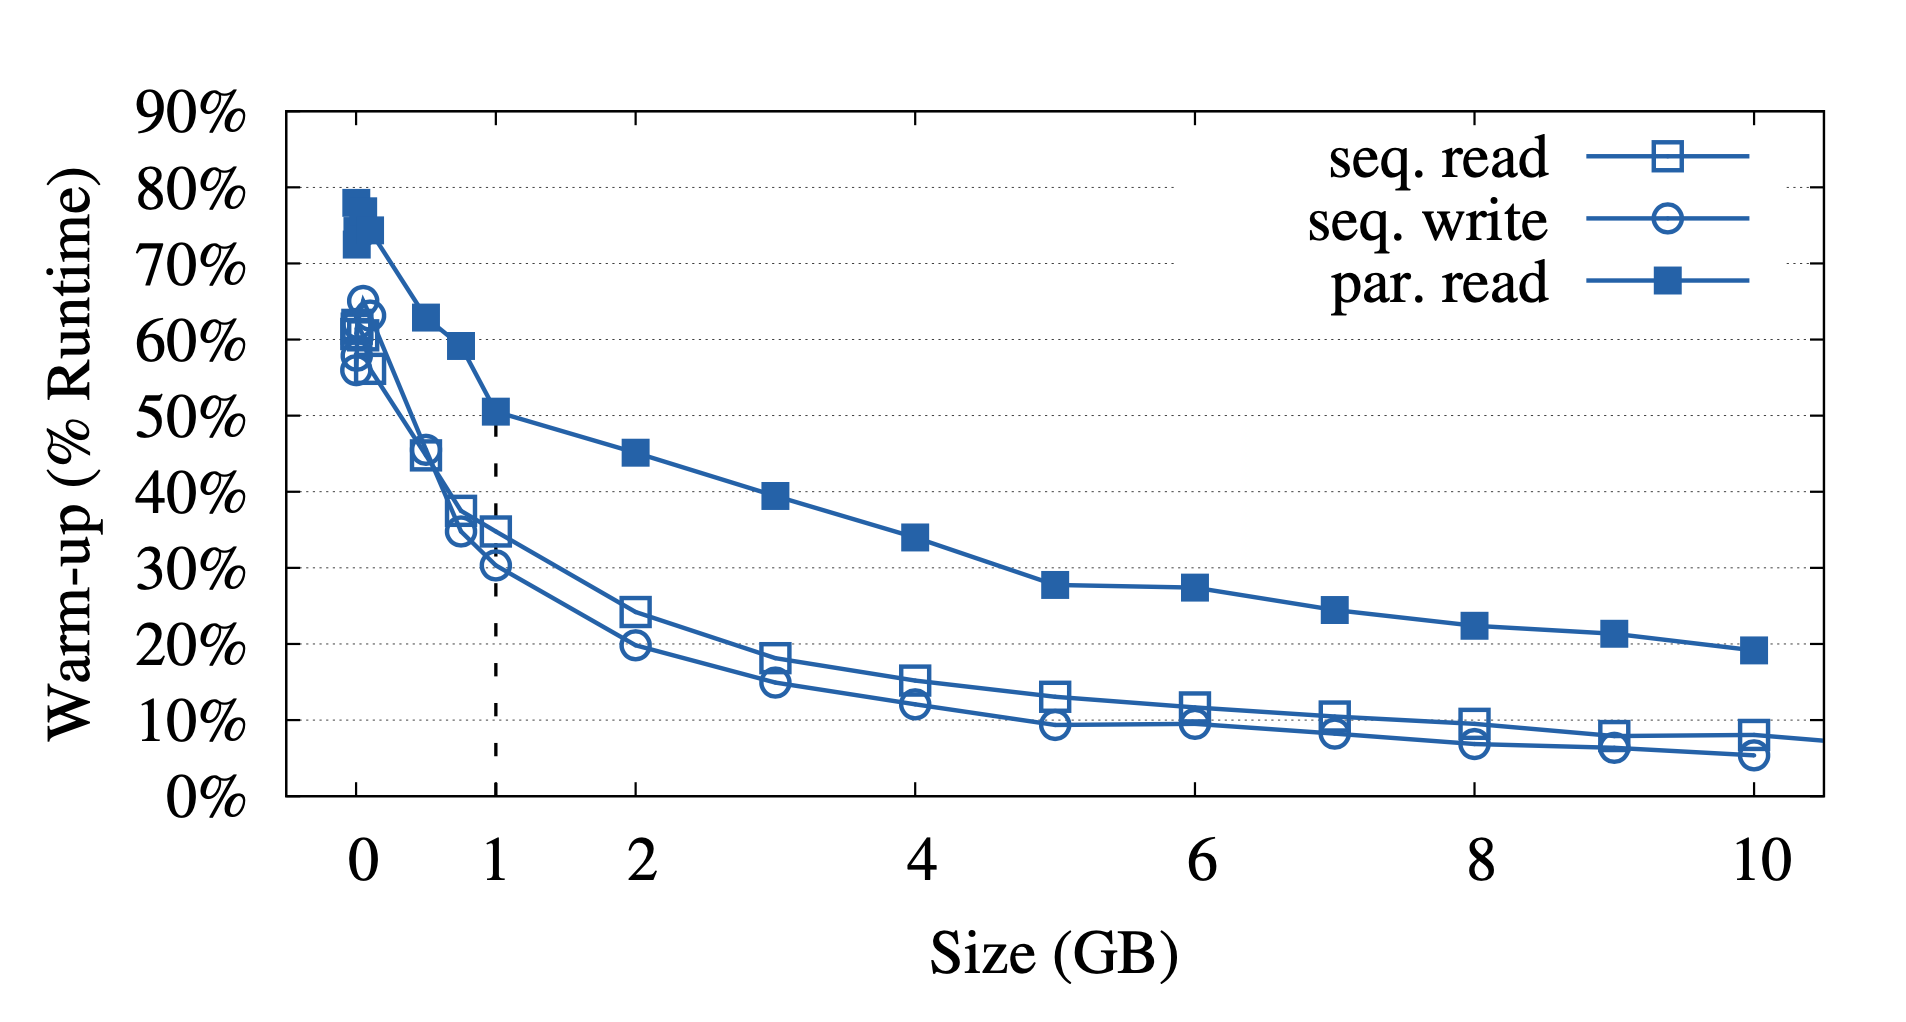
\includegraphics[width=10cm]{3-time1.png}
  \caption{HDFS请求预热耗时占运行时间百分比}
  \label{fig:time2}
\end{figure}

\paragraph{HFDS读写测试}
由于尚未有现成的HDFS测试工具,作者自己编写了sequential read,16个线程的parallel read,以及sequential write共3个客户端对HDFS性能进行分解测试。如图\ref{fig:time}所示是三个工作负载在不同的请求数据量大小下的JVM预热时间,其中int代表bytecode interpretation,而cl代表class loading。可见,JVM预热耗时不随着数据量的增大而增大,sequential write有更大的JVM预热开销,因为其运行了一条更加复杂的控制路径,使用了更多的class。图\ref{fig:time2}展示了预热时间占总运行时间的百分比,可见运行时间较短的、并行度较高的任务更容易受到JVM预热开销的影响,当数据量小于1G时,预热时间占sequential read的总运行时间的33\%以上,占parallel read运行时间的48\%以上。实际上,根据Cloudera发布的数据,真实场景下Hadoop的请求数据量小于1G,因为Hadoop将用户的请求并行化为多个较小的请求。多数用户从HDFS中读取的数据量不超过1MB,其中60\%的时间消耗在了JVM预热上。

\begin{figure}[!htp]
  \centering
  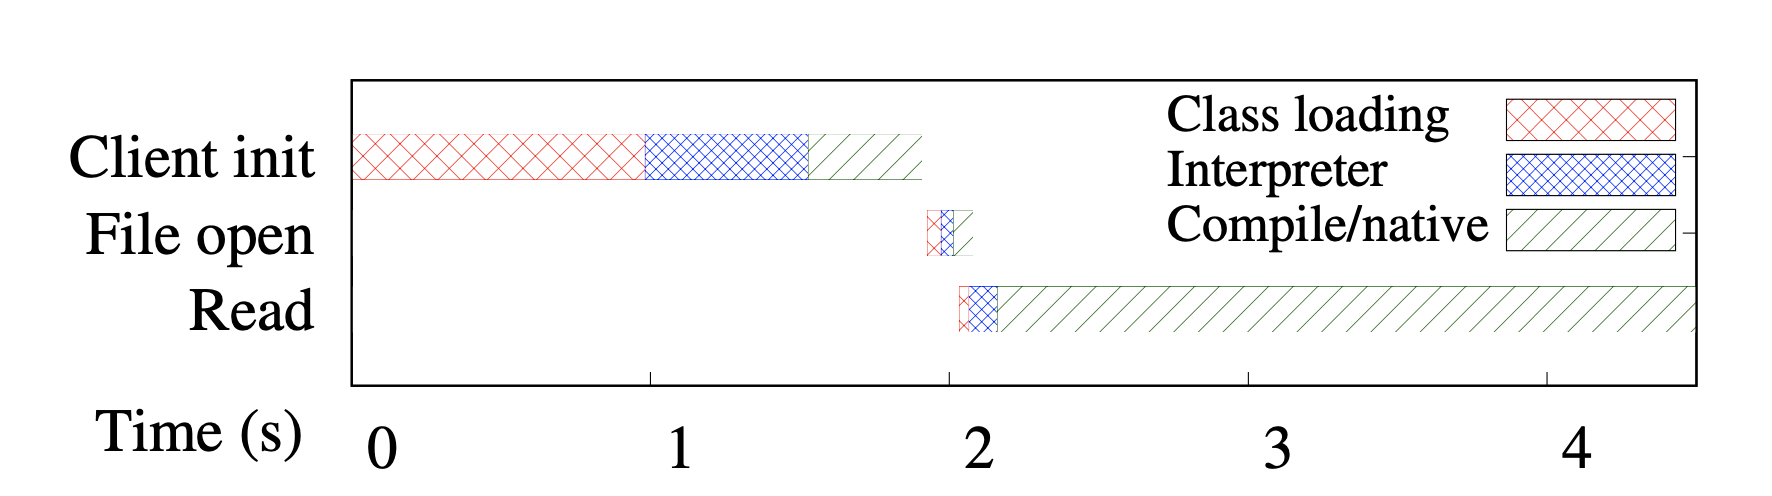
\includegraphics[width=10cm]{4-breakdown.png}
  \caption{Sequential Read 1G数据的运行时间分解}
  \label{fig:br}
\end{figure}

图\ref{fig:br}进一步展示了一个sequential read请求的整个运行过程中运行时间分解情况。可见,client端初始化时进行了较长时间的JVM预热,才开始从HDFS的datanode打开文件、读取数据。图\ref{fig:br1}进一步展示了client端和datanode端处理网络包的时间分解情况。当datanode收到了客户端的读请求之后,立刻返回了13Bytes的ack信息,继续调用sendfile系统调用发送64KB大小的数据包。如图可见,第1个sendfile花费了非常长的时间,因为需要从硬盘读取数据,而其余的数据包发送要明显快于第一个数据包。然而,客户端却由于JVM预热而无法及时相应datanode发送来的数据包,当客户端完成JVM预热并处理ack消息之后,datanode已经发送了13个数据包;再加载了处理第1个数据包所需的class、JIT编译了相关代码后,完成了第1个数据包的处理,并进行了CRC checksum的计算,花费了26ms,此时datanode已经向客户端发送了103个数据包。由此可见,I/O甚至不在I/O密集型应用的critical path上,影响I/O密集型应用性能的主要原因在于class loading和bytecode interpretation。由图\ref{fig:br1}也可以看到,解释执行的CRC checksum计算代码比JIT编译过的代码性能有巨大的差距,解释执行需要$65ms$而执行编译过的代码仅需$65\mu s$。这进一步说明了JVM预热开销的影响之大。

\begin{figure}[!htp]
  \centering
  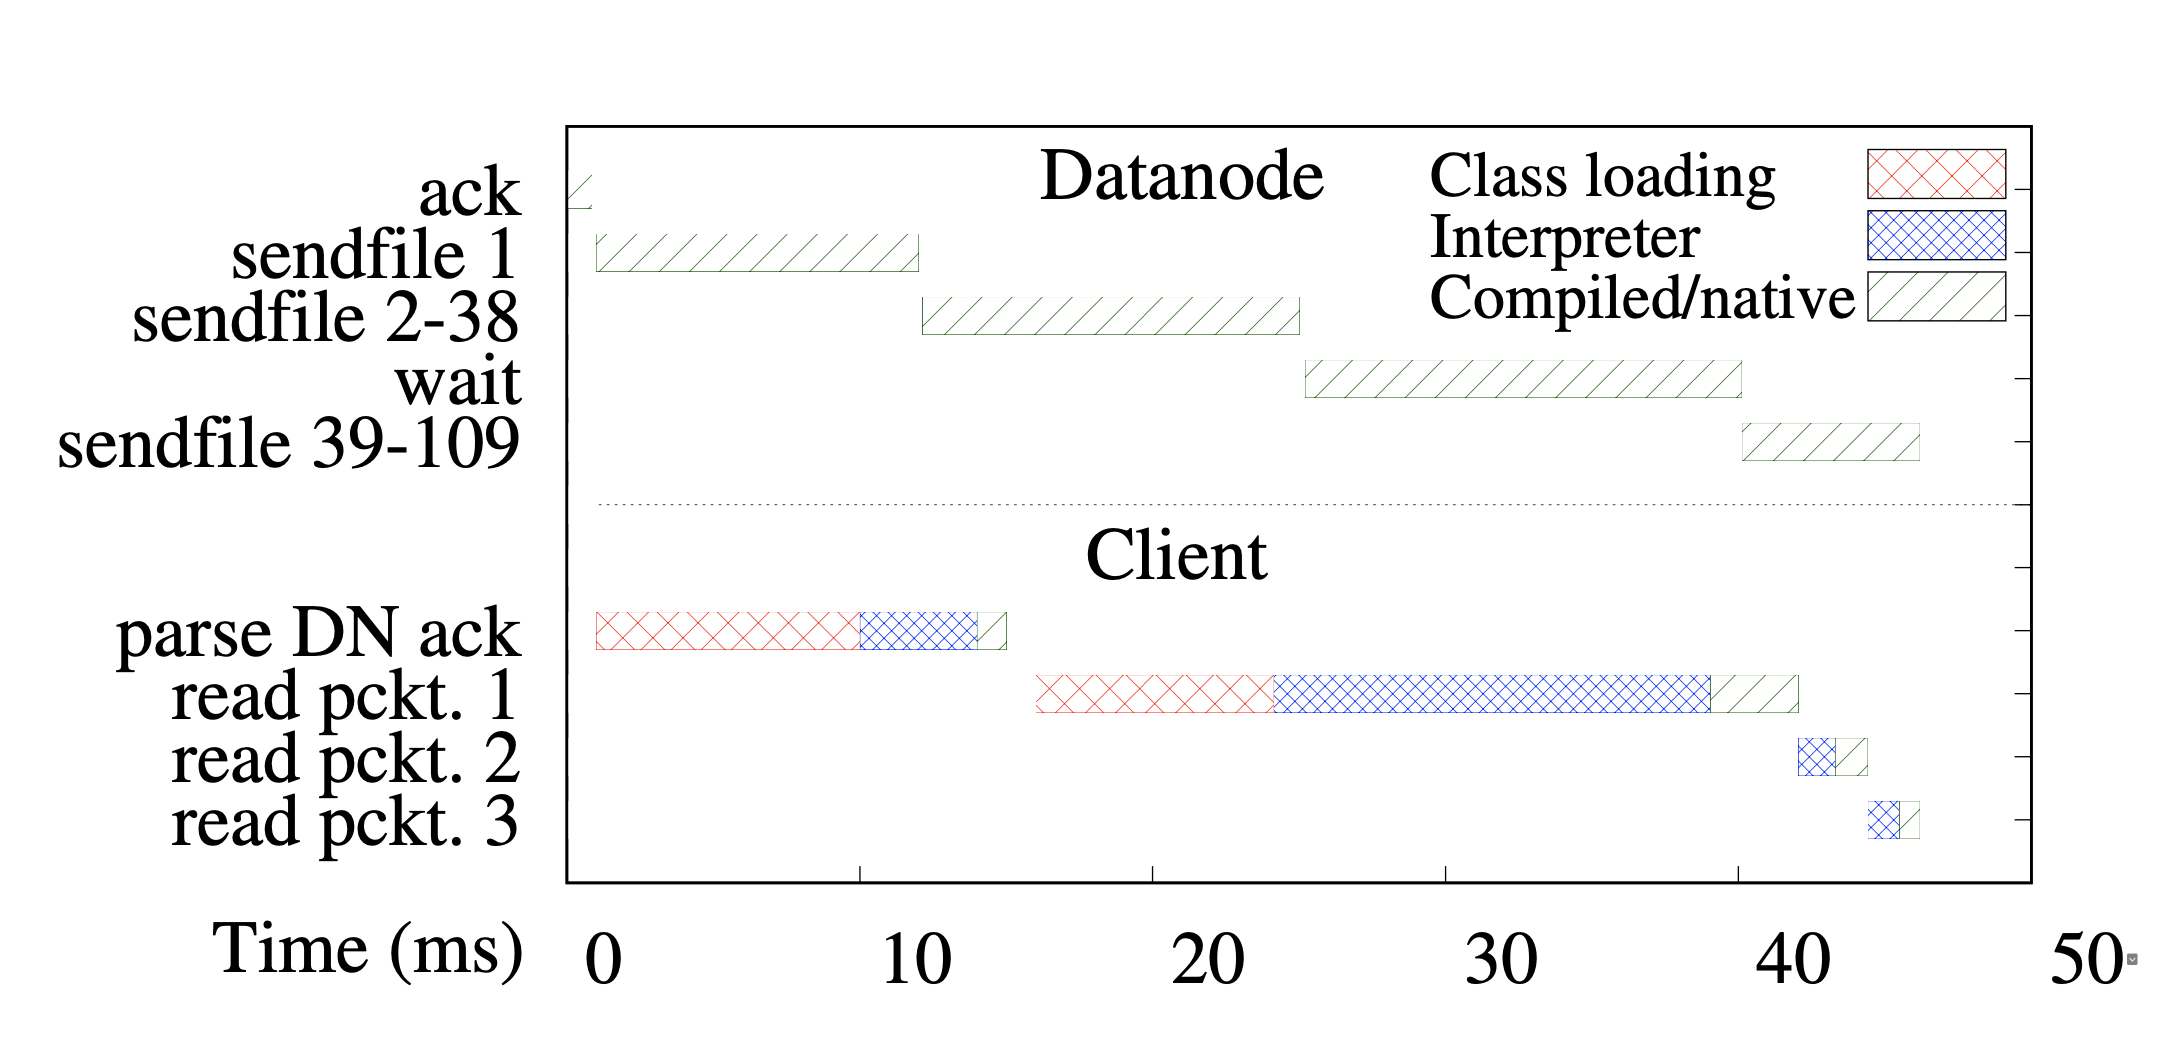
\includegraphics[width=10cm]{5-w.png}
  \caption{Datanode、client数据包传送过程时间分解}
  \label{fig:br1}
\end{figure}

\paragraph{Spark、Hive请求测试}
图\ref{fig:br2}展示了Spark、Hive处理请求的运行时间分解。Spark、Hive请求分别平均使用了21.0s和12.6秒进行了JVM预热,和HDFS测试相同,JVM预热的耗时不随着请求数据量的变化而明显变化。由于Spark依赖的软件栈较为复杂(包括来自Hadoop、Scala、derby等library的class),共计19066个class,而Hive仅需加载5855个class,故Spark的客户端在class loading上花费了6.3秒而Hive客户端仅花费了3.7秒。加载的class数量大也会导致解释执行耗时长,Spark客户端调用了242291个函数,其中91\%从未被JIT编译器编译,而Hive客户端仅调用了113944个函数,其中的96\%从未被JIT编译器编译。

\begin{figure}[!htp]
  \centering
  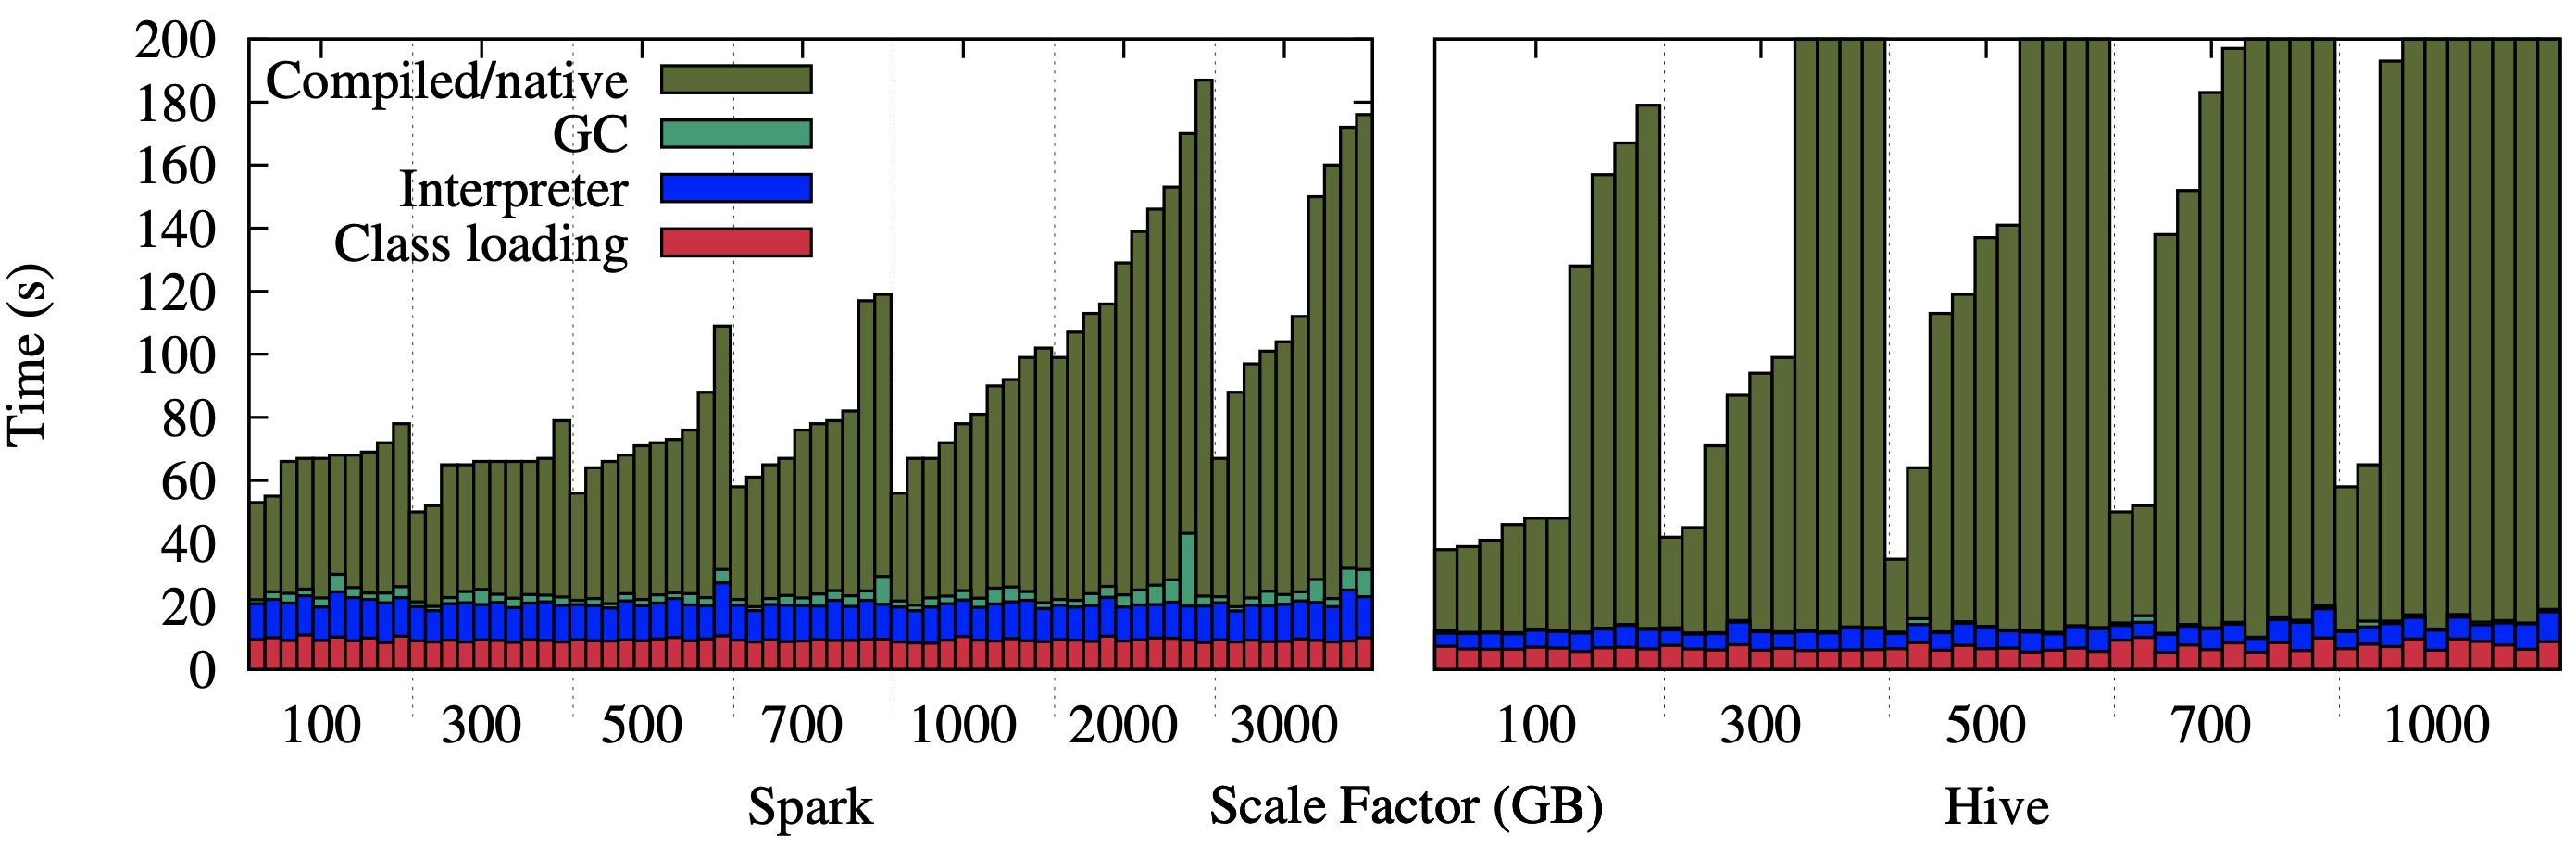
\includegraphics[width=0.9\columnwidth]{6-s.png}
  \caption{Spark、Hive请求运行时间分解}
  \label{fig:br2}
\end{figure}

图\ref{fig:br3}展示了Spark的客户端与executor(见第\ref{sec:exe}节)在进行query 13测试时的执行时间分解。由于JVM预热时间不随请求数据量的变化而显著变化,故此时间分解图有较好的代表性。整个请求花费了68s完成,其中12.4s花费在client的JVM预热,而12.2s花费在executor的JVM预热。由于client的JVM预热时间较长,executor的JVM预热时间被覆盖。但在每个iteration开始之时,executor同样经历了较长的bytecode interpretation时间。

\begin{figure}[!htp]
  \centering
  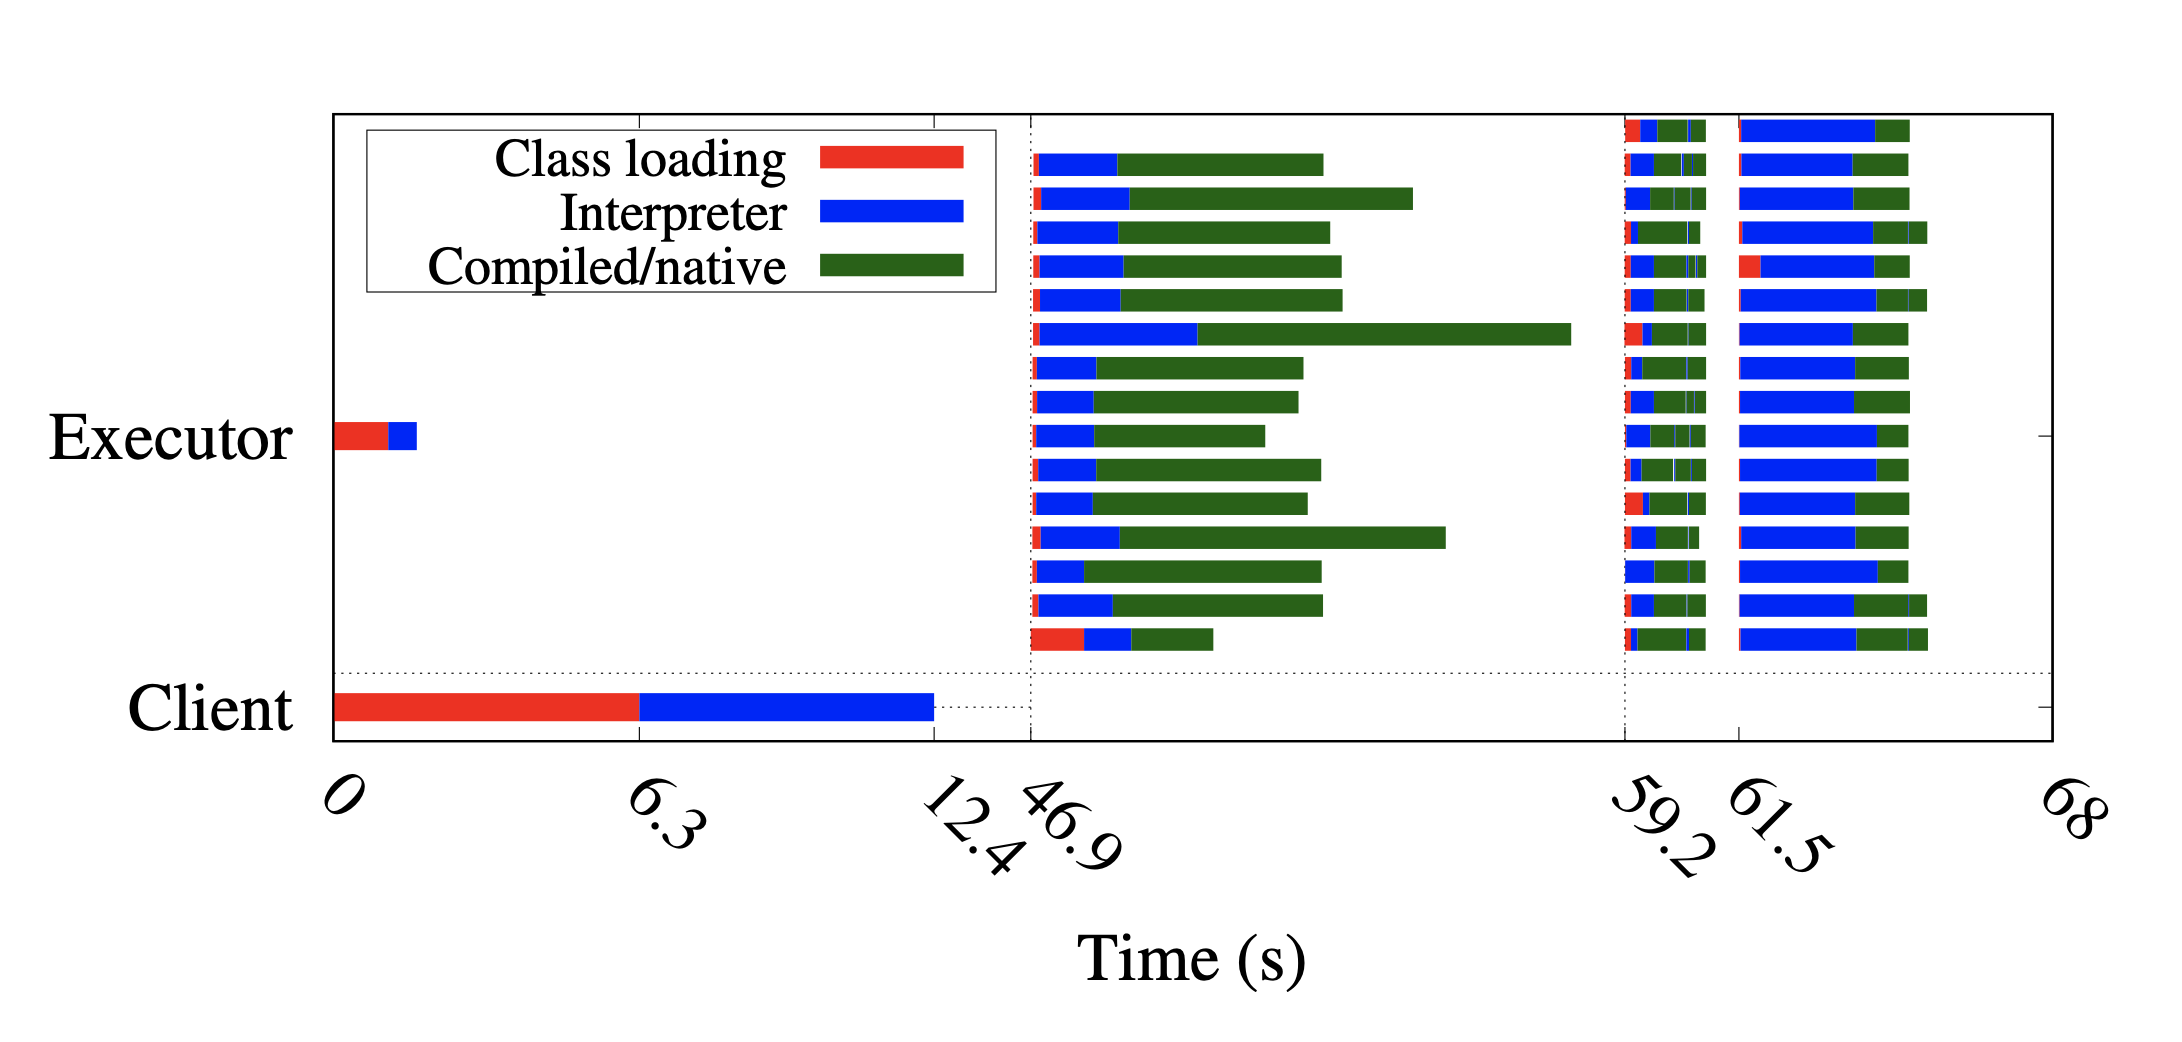
\includegraphics[width=12cm]{7-s.png}
  \caption{query 13在Spark上执行的运行时间分解}
  \label{fig:br3}
\end{figure}

Hive和Spark并行化客户请求的方式有所不同,Hive将用户的请求并行地执行在多个JVM进程中,而Spark仅有一个executor进程执行并行化的客户请求。每个JVM进程运行在container中,作为一个计算线程。然而,Hive和Tez在处理同一个用户请求的过程中会复用用一个JVM的container进程,这在一定程度上减小了JVM预热开销对性能的影响。

\paragraph{测试收获总结}
经过测试,研究者得知JVM预热耗时不随着请求数据量的变化而明显变化,同时运行时间短、并行度高的应用的运行时间会大部分地被JVM预热占据。事实上,大数据处理框架更倾向于进行运行时间短的请求,提升程序的并行度,充分利用分布式系统中充足的计算资源。复杂的分布式框架加重了JVM预热开销大的问题,因为需要加载更多的class、执行更多的不同的函数。

\subsection{HotTub设计与实现}

\subsection{HotTub性能测试}

\subsection{HotTub适用性与局限性分析}


\section{HotTub局限性优化}
// TODO

\section{总结}
// TODO

\nocite{*}
\cleardoublepage
\bibliography{wpref}

\cleardoublepage
\appendix
%\appendixpage
\addappheadtotoc
\section{附录}

\subsection{//}




\end{document}
